\chapter{Technical Solution}
\label{chap:solution}

%The DLREP function is a collection of functions proposed by \cite{Brands2000}, and used by \cite{Augot2017}. The instance generator outputs a tuple \[(q, g_1, g_2,...,g_l)\]

Using a DAC based distributed ledger is well suited for a Self-Sovereign Identity system. Using a tangle instead of a blockchain allows using a premissionless ledger, while still not monetizing the system to incentivise proof-of-work. As described in Section \ref{sec:background_dlt} the proof-of-work can be done on a per transaction basis, by utilizing the registering device's processors when an attribute is created or verified on the ledger. As double spending is not an issue when the ledger is not keeping track of ownership of value, the required proof-of-work can be adjusted to a level that is acceptable for even mobile devices.

\begin{figure}[ht]
    \centering
    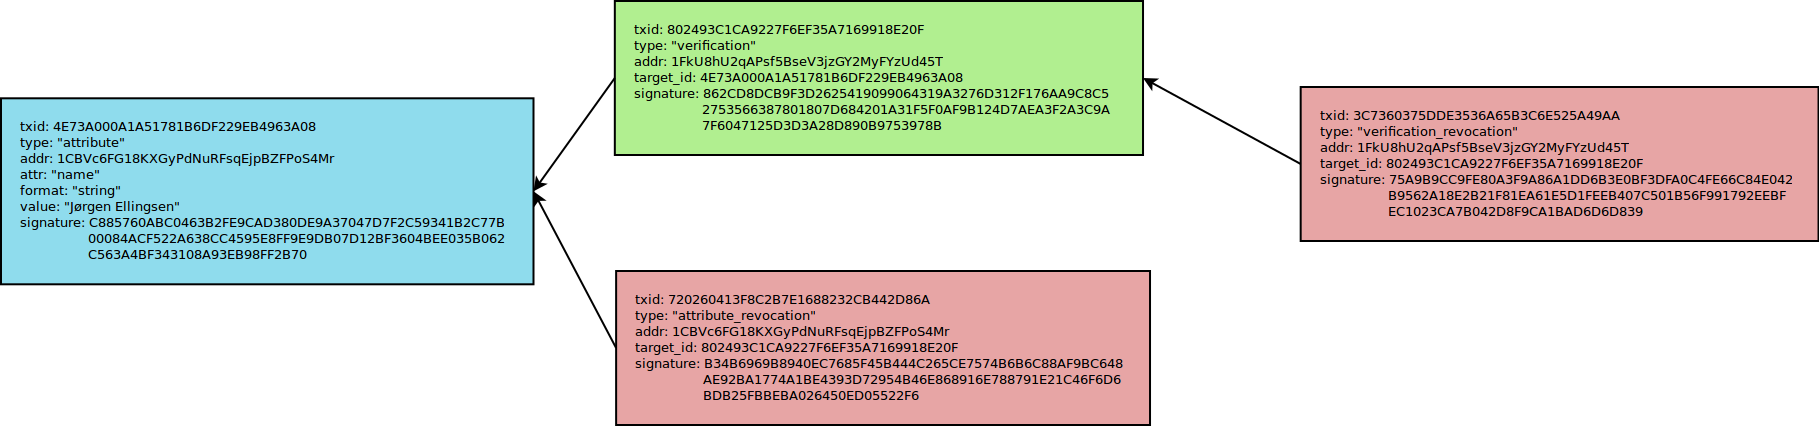
\includegraphics[width=1\textwidth]{DACSigning.png}
    \caption{Verification and Revocation}
    \label{fig:dac_sign}
\end{figure}
